\documentclass[12pt,twoside]{article}

\textwidth 17cm \textheight 25cm \evensidemargin 0cm
\oddsidemargin 0cm \topmargin -2cm
\parindent 0pt
%\parskip \bigskipamount

\usepackage{graphicx}
\usepackage[dutch]{babel}
\usepackage{amssymb,amsthm,amsmath}
%\usepackage{dot2texi}
\usepackage[utf8]{inputenc}
\usepackage{nopageno}
\usepackage{pdfpages}
\usepackage{enumerate}
\usepackage{caption}
\usepackage{wrapfig}
\usepackage{pgf,tikz,pgfplots}
\pgfplotsset{compat=1.15}
\usepackage{color}
\usetikzlibrary{arrows}
\usetikzlibrary{patterns}
\usepackage{fancyhdr}
\pagestyle{fancy}
\usepackage[version=3]{mhchem}
\usepackage{multicol}
\usepackage{fix-cm}
\usepackage{setspace}
\usepackage{mhchem}
\usepackage{xhfill}
\usepackage{parskip}
\usepackage{cancel}
\usepackage{mdframed}
\usepackage{url}
\usepackage{mathtools}
\usepackage{changepage}

\newcommand{\todo}[1]{{\color{red} TODO: #1}}

\newcommand{\degree}{\ensuremath{^\circ}}
\newcommand\rad{\qopname\relax o{\mathrm{rad}}}

\newcommand\ggd{\qopname\relax o{\mathrm{ggd}}}

\pgfmathdeclarefunction{gauss}{2}{%
  \pgfmathparse{1/(#2*sqrt(2*pi))*exp(-((x-#1)^2)/(2*#2^2))}%
}

\def\LRA{\Leftrightarrow}

\newcommand{\zrmbox}{\framebox{\phantom{EXE}}\phantom{X}}
\newcommand{\zrm}[1]{\framebox{#1}}

% environment oefening:
% houdt een teller bij die de oefeningen nummert, probeert ook de oefening op één pagina te houden
\newcounter{noefening}
\setcounter{noefening}{0}
\newenvironment{oefening}
{
  \stepcounter{noefening}
  \pagebreak[0]
  \begin{minipage}{\textwidth}
  \vspace*{0.7cm}{\large\bf Oefening \arabic{noefening}}
}{%
  \end{minipage}
}

\usepackage{calc}

% vraag
\reversemarginpar
\newcounter{punten}
\setcounter{punten}{0}
\newcounter{nvraag}
\setcounter{nvraag}{1}
\newlength{\puntwidth}
\newlength{\boxwidth}
\newcommand{\vraag}[1]{
\settowidth{\puntwidth}{\Large{#1}}
\setlength{\boxwidth}{1.5cm}
\addtolength{\boxwidth}{-\puntwidth}
{\large\bf Vraag \arabic{nvraag} \addtocounter{nvraag}{1}}\vspace*{-0.5cm}
{\marginpar{\color{lightgray}\fbox{\parbox{1.5cm}{\vspace*{1cm}\hspace*{\boxwidth}{\Large{#1}}}}}
\vspace*{0.5cm}}
\addtocounter{punten}{#1}}

% arulefill
\def\arulefill{\leavevmode{\xrfill[-5pt]{0.3pt}[lightgray]\endgraf}\vspace*{0.2cm}}

% \arules{n}
\newcommand{\arules}[1]{
\color{lightgray}
%\vspace*{0.05cm}
\foreach \n in {1,...,#1}{
  \vspace*{0.75cm}
  \hrule height 0.3pt\hfill
}\color{black}\vspace*{0.2cm}}

% \arule{x}
\newcommand{\arule}[1]{
\color{lightgray}{\raisebox{-0.1cm}{\rule[-0.05cm]{#1}{0.3pt}}}\color{black}
}

% \abox{y}
\newcommand{\abox}[1]{
\fbox{
\begin{minipage}{\textwidth- 4\fboxsep}
\hspace*{\textwidth}\vspace{#1}
\end{minipage}
}
}

\newcommand{\ruitjes}[1]{
\definecolor{cqcqcq}{rgb}{0.85,0.85,0.85}
\hspace*{-2.5cm}
\begin{tikzpicture}[scale=1.04,line cap=round,line join=round,>=triangle 45,x=1.0cm,y=1.0cm]
\draw [color=cqcqcq, xstep=0.5cm, ystep=0.5cm] (0,-#1) grid (20.5,0);
\end{tikzpicture}
}


\newcommand{\assenstelsel}[5][1]{
\definecolor{cqcqcq}{rgb}{0.65,0.65,0.65}
\begin{tikzpicture}[line cap=round,line join=round,>=triangle 45,x=#1cm,y=#1cm]
\draw [color=cqcqcq,dash pattern=on 1pt off 1pt, xstep=1.0cm,ystep=1.0cm] (#2,#4) grid (#3,#5);
\draw[->,color=black] (#2,0) -- (#3,0);
%\draw[shift={(1,0)},color=black] (0pt,2pt) -- (0pt,-2pt) node[below] {\footnotesize $1$};
%\draw[color=black] (#3.25,0.07) node [anchor=south west] {$x$};
\draw[->,color=black] (0,#4) -- (0,#5);
%\draw[shift={(0,1)},color=black] (2pt,0pt) -- (-2pt,0pt) node[left] {\footnotesize $1$};
\draw[color=black] (0.09,#5.25) node [anchor=west] {\phantom{$y$}};
%\draw[color=black] (0pt,-10pt) node[right] {\footnotesize $0$};
\end{tikzpicture}
}

\newcommand{\getallenas}[3][1]{
\definecolor{cqcqcq}{rgb}{0.65,0.65,0.65}
\begin{tikzpicture}[scale=#1,line cap=round,line join=round,>=triangle 45,x=1.0cm,y=1.0cm]
\draw [color=cqcqcq,dash pattern=on 1pt off 1pt, xstep=1.0cm,ystep=1.0cm] (#2,-0.2) grid (#3,0.2);
\draw[->,color=black] (#2.25,0) -- (#3.5,0);
\draw[shift={(0,0)},color=black] (0pt,2pt) -- (0pt,-2pt) node[below] {\footnotesize $0$};
\draw[shift={(1,0)},color=black] (0pt,2pt) -- (0pt,-2pt) node[below] {\footnotesize $1$};
\draw[color=black] (#3.25,0.07) node [anchor=south west] {$\mathbb{R}$};
\end{tikzpicture}
}

\newcommand{\visgraad}[1]{\begin{tabular}{p{0.5cm}|p{#1}}&\\\hline\\\end{tabular}}

\newcommand{\tekenschema}[2]{\begin{tabular}{p{0.5cm}|p{#1}}&\\\hline\\[#2]\end{tabular}}

% schema van Horner
\newcommand{\schemahorner}{
\begin{tabular}{p{0.5cm}|p{7cm}}
&\\[1.5cm]
\hline\\
\end{tabular}}

% geef tabular iets meer ruimte
\setlength{\tabcolsep}{14pt}
\renewcommand{\arraystretch}{1.5}

\newcommand{\toets}[3]{
\thispagestyle{plain}
\vspace*{-2.5cm}
\begin{tikzpicture}[remember picture, overlay]
    \node [shift={(15.25 cm,-1.6cm)}] {%
        \includegraphics[width=1.8cm]{/home/ppareit/kaa1415/logokaavelgem.png}%
    };%
\end{tikzpicture}

\begin{tabular}{|llc|c|}
\hline
\vspace*{-0.5cm}
&&&\\
Naam & \arule{4cm} & {\Large\bf KA AVELGEM} & \\
\vspace*{-0.75cm}
&&&\\
Klas & \arule{4cm} & {\Large\bf 20...-...-...} & \\
\hline
\vspace*{-0.75cm}
&&&\\
Toets & {\bf #2} & {\large\bf #1} & Beoordeling\\
\vspace*{-0.75cm}
&&&\\
Onderwerp & \multicolumn{2}{l|}{\bf #3} &\\
\hline
\end{tabular}
}

\newcommand{\oefeningen}[1]{

\fancyhead[LE, RO]{\vspace{0.5cm} #1}
%\thispagestyle{plain}

{\bf \Large \centering Oefeningen: #1}

}

\raggedbottom

\newcommand\vl{\qopname\relax o{\mathrm{vl}}}

\newcommand\dom{\qopname\relax o{\mathrm{dom}}}
\newcommand\ber{\qopname\relax o{\mathrm{ber}}}

\newcommand\mC{\qopname\relax o{\mathrm{mC}}}
\newcommand\uC{\qopname\relax o{\mathrm{{\mu}C}}}
\newcommand\C{\qopname\relax o{\mathrm{C}}}

\newcommand\W{\qopname\relax o{\mathrm{W}}}
\newcommand\kW{\qopname\relax o{\mathrm{kW}}}
\newcommand\kWh{\qopname\relax o{\mathrm{kWh}}}


\newcommand\V{\qopname\relax o{\mathrm{V}}}
\newcommand\ohm{\qopname\relax o{\mathrm{\Omega}}}
\newcommand\kohm{\qopname\relax o{\mathrm{k\Omega}}}


\newcommand\N{\qopname\relax o{\mathrm{N}}}

\newcommand\Nperkg{\qopname\relax o{\mathrm{N/kg}}}

\newcommand\Nperm{\qopname\relax o{\mathrm{N/m}}}

\newcommand\gpermol{\qopname\relax o{\mathrm{g/mol}}}


\newcommand\kgperm{\qopname\relax o{\mathrm{kg/m}}}
\newcommand\kgperdm{\qopname\relax o{\mathrm{kg/dm}}}
\newcommand\gpercm{\qopname\relax o{\mathrm{g/cm}}}
\newcommand\gperml{\qopname\relax o{\mathrm{g/ml}}}


\newcommand{\mA}{\;\mbox{mA}}
\newcommand{\A}{\;\mbox{A}}
\newcommand{\MA}{\;\mbox{MA}}

\newcommand{\us}{\;\mu\mbox{s}}
\newcommand\s{\qopname\relax o{\mathrm{s}}}

\newcommand\h{\qopname\relax o{\mathrm{h}}}

\newcommand{\kmperh}{\;\mbox{km/h}}
\newcommand{\mpers}{\;\mbox{m/s}}
\newcommand{\kmpermin}{\;\mbox{km/min}}
\newcommand{\kmpers}{\;\mbox{km/s}}

\newcommand{\mph}{\;\mbox{mph}}

\newcommand{\Hz}{\;\mbox{Hz}}

\newcommand\Gm{\qopname\relax o{\mathrm{Gm}}}
\newcommand\Mm{\qopname\relax o{\mathrm{Mm}}}
\newcommand\km{\qopname\relax o{\mathrm{km}}}
\newcommand\hm{\qopname\relax o{\mathrm{hm}}}
\newcommand\dam{\qopname\relax o{\mathrm{dam}}}
\newcommand\m{\qopname\relax o{\mathrm{m}}}
\newcommand\dm{\qopname\relax o{\mathrm{dm}}}
\newcommand\cm{\qopname\relax o{\mathrm{cm}}}
\newcommand\mm{\qopname\relax o{\mathrm{mm}}}
\newcommand\um{\qopname\relax o{\mathrm{{\mu}m}}}
\newcommand\nm{\qopname\relax o{\mathrm{nm}}}


\newcommand\Gg{\qopname\relax o{\mathrm{Gg}}}
\newcommand\Mg{\qopname\relax o{\mathrm{Mg}}}
\newcommand\kg{\qopname\relax o{\mathrm{kg}}}
\newcommand\hg{\qopname\relax o{\mathrm{hg}}}
\renewcommand\dag{\qopname\relax o{\mathrm{dag}}}
\newcommand\g{\qopname\relax o{\mathrm{g}}}
\newcommand\dg{\qopname\relax o{\mathrm{dg}}}
\newcommand\cg{\qopname\relax o{\mathrm{cg}}}
\newcommand\mg{\qopname\relax o{\mathrm{mg}}}
\newcommand\ug{\qopname\relax o{\mathrm{{\mu}g}}}
\renewcommand\ng{\qopname\relax o{\mathrm{ng}}}

\newcommand\ton{\qopname\relax o{\mathrm{ton}}}

\newcommand\Gl{\qopname\relax o{\mathrm{Gl}}}
\newcommand\Ml{\qopname\relax o{\mathrm{Ml}}}
\newcommand\kl{\qopname\relax o{\mathrm{kl}}}
\newcommand\hl{\qopname\relax o{\mathrm{hl}}}
\newcommand\dal{\qopname\relax o{\mathrm{dal}}}
\renewcommand\l{\qopname\relax o{\mathrm{l}}}
\newcommand\dl{\qopname\relax o{\mathrm{dl}}}
\newcommand\cl{\qopname\relax o{\mathrm{cl}}}
\newcommand\ml{\qopname\relax o{\mathrm{ml}}}
\newcommand\ul{\qopname\relax o{\mathrm{{\mu}l}}}
\newcommand\nl{\qopname\relax o{\mathrm{nl}}}

\newcommand\MJ{\qopname\relax o{\mathrm{MJ}}}
\newcommand\kJ{\qopname\relax o{\mathrm{kJ}}}
\newcommand\J{\qopname\relax o{\mathrm{J}}}

\newcommand\T{\qopname\relax o{\mathrm{T}}}
\newcommand\uT{\qopname\relax o{\mathrm{{\mu}T}}}

\newcommand\grC{\qopname\relax o{\mathrm{{\degree}C}}}

\newcommand\K{\qopname\relax o{\mathrm{K}}}
\newcommand\calperK{\qopname\relax o{\mathrm{cal/K}}}

\newcommand\hPa{\qopname\relax o{\mathrm{hPa}}}
\newcommand\Pa{\qopname\relax o{\mathrm{Pa}}}

\newcommand\dB{\qopname\relax o{\mathrm{dB}}}

\newcommand\Var{\qopname\relax o{\mathrm{Var}}}

\newcommand{\EE}[1]{\cdot 10^{#1}}

\onehalfspacing

%\setlength{\headsep}{0cm}

\newenvironment{exlist}[1] %
{ \begin{multicols}{#1}
  \begin{enumerate}[(a)]
    \setlength{\itemsep}{0.5em} }
{ \end{enumerate}
  \end{multicols} }




\usepackage{versions}
%\excludeversion{theorie}
\includeversion{theorie}

\begin{document}

\pagestyle{fancy}
\lhead{}
\rhead{Oefeningen Exponentiële Functies}

\begin{theorie}

  \thispagestyle{empty}
  \begin{center}
    \begin{mdframed}
      \centering
      \fontsize{40}{60}\selectfont Exponentiële functies
    \end{mdframed}
    \vfill
    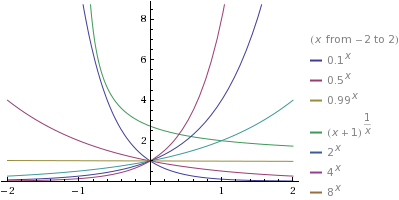
\includegraphics{exp_func} %TODO: replace
    \vfill
  \end{center}

  \subsection*{Doelstellingen}
  \vspace*{-0.8cm}
  {\singlespacing
    Je \hfill  {\scriptsize(LP2006-059, LI1.9, ET32,14,31)}
    \begin{itemize}
      \itemsep-0.2em
      \item kan n-de wortel berekenen in $\mathbb{R}$
      \item kent de definitie van een macht met een rationale exponent en kunnen de elementaire rekenregels toepassen
      \item kan voor geschikte domeinen een verband leggen tussen de onderstaande functies en conclusies trekken in verband met hun grafieken:
      \begin{itemize}
        \item $x^2$ en $\sqrt{x}$
        \item $x^3$ en $\sqrt[3]{x}$
        \item $x^n$ en $\sqrt[n]{x}$
      \end{itemize}
      \item kent de definitie van een exponentiële functie $f(x)=a^x$
      \item kan het onderscheid tussen een lineair en een exponentieel groeiproces
      \item kunt van een exponentiële functie de de tabel, de grafiek, het domein, enkele bijzondere waarden, het stijgen/dalen en het asymptotisch gedrag bepalen, eventueel met behulp van ICT
      \item kunt aan de hand van de grafiek het domein, het bereik, de bijzondere waarden, het tekenverloop, het stijgen/dalen en het asymptotisch gedrag bepalen van exponentiële functies
    \end{itemize}}

  \thispagestyle{empty}
  \mbox{}
  \newpage
  \clearpage
  \thispagestyle{empty}
  % \mbox{}
  \tableofcontents
  \newpage
  \clearpage
  \pagenumbering{arabic} 

  \fancyhead[RO,LE]{Irrationale functies}
  \fancyhead[RE,LO]{}

\end{theorie}

\section{Machten met gehele exponenten}

\begin{oefening}
Geef de definitie van een macht met een natuurlijke exponent.
\end{oefening}

\begin{oefening}
Bespreek het teken van machten met een natuurlijke exponent.
\end{oefening}

\begin{oefening}
Geef de definitie van een macht met een negatieve exponent.
\end{oefening}

\begin{oefening}*
Leid volgende eigenschappen van de machtsverheffing af:
\begin{align*}
  a^m a^n &= a^{m+n} && \mbox{product van machten}\\
  \dfrac{a^m}{a^n} &= a^{m-n} && \mbox{quotiënt van machten}\\
  \left(a^m\right)^n &= a^{m\cdot n} && \mbox{macht van een macht}\\
  \left(ab\right)^n &= a^n b^n && \mbox{macht van een product}\\
  \left(\dfrac{a}{b}\right)^n &= \dfrac{a^n}{b^n} && \mbox{macht van een quotiënt}
\end{align*}
\end{oefening}

\begin{oefening}
Bereken zonder \zrm{ZRM}.
\begin{multicols}{4}
  \begin{enumerate}[(a)]
    \itemsep.5em
    \item $5^2$
    \item $5^3$
    \item $(-5)^2$
    \item $(-5)^3$
    \item $-5^2$
    \item $-5^3$
    \item $5^{-2}$
    \item $5^{-3}$
    \item $-5^{-2}$
    \item $-5^{-3}$
    \item $(-5)^{-2}$
    \item $(-5)^{-3}$
  \end{enumerate}
\end{multicols}
\end{oefening}

\begin{oefening}
Bereken en controleer nadien met het \zrm{ZRM}.
\begin{multicols}{4}
\begin{enumerate}[(a)]
  \itemsep.5em
  \item $\left(-3\right)^0$
  \item $\left(-4\right)^1$
  \item $\left(\dfrac{1}{3}\right)^5:\dfrac{1}{3}$
  \item $\left(\dfrac{4}{5}\right)^{-1}$
  \item $\left(-\dfrac{1}{6}\right)^{-3}$
  \item $\left(\dfrac{2}{5}\right)^{-2}$
  \item $2^{-1}$
  \item $\left(-\dfrac{2}{5}\right)^{-2}$
  \item $\left[\left(-1\right)^6\right]^3$
  \item $[-1^6]^3$
  \item $\dfrac{0.8^{-3}}{0.8^{-6}}$
  \item $\dfrac{\left(-4\right)^{0}}{\left(-4\right)^{-2}}$
  \item $[\left(-0.1\right)^2]^3$
  \item $\left(\sqrt{2}\right)^{-2}$
  \item $1.1^2$
  \item $0.3^{-2}$
  \item $\left(-0.01\right)^{-5}$
  \item $\left(-0.05\right)^{-1}$
  \item $0.2^{-4}$
  \item $0.08^{-3}$
  \item $0.5^{-2}\cdot0.5^{-3}$
  \item $\left(-2\cdot2^{-2}\right)^{-2}$
  \item $\dfrac{1}{\left(\sqrt{2}\right)}^{-2}$
\end{enumerate}
\end{multicols}
\end{oefening}

\begin{oefening}
Bereken volgende machten zonder \zrm{ZRM}. Maak steeds een tussenstap.
\begin{multicols}{3}
  \begin{enumerate}[(a)]
    \itemsep.5em
    \item $-(-2)^3$
    \item $-(-3)^2$
    \item $-2^{-3}$
    \item $3^{-2}$
    \item $(-2)^{-4}$
    \item $(-2)^{-5}$
    \item $(-1)^{802}$
    \item $-(-604)^{0}$
    \item $\left(-\dfrac{\sqrt{7}}{8\pi}\right)^{0}$
    \item $2.5^{2}$
    \item $0.04^{3}$
    \item $\left(-\dfrac{6}{11}\right)^{2}$
    \item $\left(-\dfrac{4}{5}\right)^{3}$
    \item $\left(-\dfrac{1}{3}\right)^{-3}$
    \item $\left(\dfrac{2}{7}\right)^{-2}$
    \item $\left(\sqrt{2}\right)^{2}$
    \item $\left(\sqrt{2}\right)^{4}$
    \item $\left(\sqrt{2}\right)^{-1}$
    \item $(-0.01)^{-4}$
    \item $\left(-\dfrac{1}{\sqrt{5}}\right)^{1}$
    \item $\left(-\dfrac{5}{\sqrt{2}}\right)^{-2}$
    \item $\left(\dfrac{\sqrt{2}}{3}\right)^{-4}$
    \item $\left(-\dfrac{1}{\sqrt{3}}\right)^{-6}$
    \item $\left(-\dfrac{45}{60}\right)^{3}$
    \item $(1.5)^{-2}$
    \item $\dfrac{1}{4^{-2}}$
  \end{enumerate}
\end{multicols}
\end{oefening}

\begin{oefening}
Vereenvoudig:
\begin{multicols}{3}
  \begin{enumerate}[(a)]
  \itemsep.5em
  \item $a^2\cdot a^3$
  \item $a^2+a^3$
  \item $a^9\cdot2^{-5}$
  \item $\dfrac{a^8}{\left({a^2}\right)^4}$
  \item $\left(a^8\right)^2$
  \item $\left(\dfrac{a^2}{b^4}\right)^{-2}$
  \end{enumerate}
\end{multicols}
\end{oefening}

\begin{oefening}
Schrijf zo eenvoudig mogelijk.
\begin{multicols}{3}
\begin{enumerate}[(a)]
  \itemsep.5em
  \item $a^2\cdot a^8$
  \item $a^4\cdot a^{-2}$
  \item $x^2\cdot y^2$
  \item $a^2b^3c^4a^{-2}b^{-3}c^{-4}$
  \item $a^2a^2-a^4$
  \item $\dfrac{a^0}{b^0}$
  \item $\dfrac{a^1}{b^2}$
  \item $a^2+a^2$
  \item $a^2+a^3$
  \item $\dfrac{a^3}{a^2}$
  \item $\dfrac{a^{-10}}{a^{-5}}\cdot{a^3}$
  \item $\dfrac{x^2y^1z^0}{x^{-2}y^{-1}z^{0}}$
  \item $4^a+2^{2a}$
  \item $4^a\cdot2^{2a}$
  \item $\frac{2a\cdot a^{2}}{a^{3}}$
  \item $\left(-a^4\right)\cdot\left(+a^4\right)$
  \item $\left(-a^4\right):\left(+a^4\right)$
  \item $\left(-0.5ab^2\right)^3$
  \item $\left(\left(xy\right)^4y\right)^{-2}$
  \item $\left(\dfrac{2a}{b^{-2}}\right)^2$
\end{enumerate}
\end{multicols}
\end{oefening}

\begin{oefening}
Werk uit:
\begin{multicols}{3}
  \begin{enumerate}[(a)]
  \itemsep.5em
    \item $2^3\cdot 2^2$
    \item $10^4\cdot 10^2$
    \item $\left(\dfrac{2}{3}\right)\cdot \left(\dfrac{2}{3}\right)^2$
    \item $2^8\cdot 2^{-6}$
    \item $\left(-2\right)^4\cdot \left(-2\right)^{-4}$
    \item $\left(-\frac{1}{2}\right)^{-4}\cdot \left(-\frac{1}{2}\right)^2$
    \item $8^4\cdot 8\cdot 8^{-6}$
    \item $0.3\cdot 0.3^5\cdot 0.3^{-3}$
    \item $2^5: 2^2$
    \item $10^3: 10^2$
    \item $\left(\dfrac{3}{4}\right)^3: \left(\dfrac{3}{4}\right)$
    \item $3^{-2}: 3^3$
    \item $\dfrac{10^{-1}}{10^{-3}}$
    \item $\dfrac{2^{3}}{2^{7}}$
    \item $\dfrac{(-2)^{-5}}{(-2)^{-2}}$
    \item $3.2^{-1}:3.2^{-3}$
    \item $6^2\cdot 6^{-3}$
    \item $\dfrac{9^4}{9^2}$
    \item $\left(-3\right)^{-1}\cdot \left(-3\right)^3$
    \item $\dfrac{\left(-1\right)^{-4}}{\left(-1\right)^{-1}}$
    \item $4^3\cdot 4^{-6}$
    \item $\dfrac{\left(-5\right)^{-3}}{\left(-5\right)^{-1}}$
    \item $10^3\cdot 10^{-3}$
    \item $\dfrac{-3^3}{3^4}$
    \item $1^4\cdot1\cdot1^{-6}$
    \item $\dfrac{\left(-3\right)^{2}}{\left(-3\right)^{4}}$
%    \item $10^2-1^2$
%    \item $\left(-1\right)^6\cdot \left(-1\right)^{-3}$
%    \item $\dfrac{7^{3}}{7^{5}}$
%    \item $\left(-5\right)^4\cdot \left(-5\right)^{-2}$
%    \item $\dfrac{1.4^{-3}}{1.4^{-2}}$
%    \item $\left(-2\right)^4\cdot \left(-2\right)^{-6}$
  \end{enumerate}
\end{multicols}
\end{oefening}

\begin{oefening}
Noteer korter, indien mogelijk.
\begin{multicols}{3}
  \begin{enumerate}[(a)]
    \itemsep1.5em
    \item $x\cdot x\cdot x$
    \item $x+x+x$
    \item $a^5\cdot a^2$
    \item $b^7\cdot b^3\cdot b^8$
    \item $\left(-x^2\right)\left(-x^2\right)$
    \item $-x^2-x^2-x^2$
    \item $a\cdot a^6$
    \item $\left(x^5\right)^2$
    \item $\left(a^3\right)^3$
    \item $\left(-x^3\right)^2$
    \item $\left(x^2\right)^3$
    \item $a^8\cdot a^{-4}$
    \item $\left(-a^{-2}\right)^3$
    \item $a^4+a^4$
    \item $\left(a^4\right)^2\left(a^3\right)^5$
    \item $a^2\left(a^7\right)^3\left(a^4\right)^2$
    \item $ab^2+ab^2+ab^2$
    \item $ab^2\cdot ab^2\cdot ab^2$
    \item $\left(-x^3\right)^2\left(-x^2\right)^3$
    \item $\left(abc\right)^2\left(2bc\right)^3$
    \item $a^{-3}\cdot a$
    \item $\left(5a\right)^{-2}$
    \item $\left(\dfrac{-3}{y}\right)^{-3}$
    \item $\dfrac{\left(6a^3\right)^2}{\left(-3a\right)^3}$
    \item $ab^-2:bz^-2$
  \end{enumerate}
\end{multicols}
\end{oefening}

\begin{oefening}
Werk zo ver mogelijk uit en schrijf de uitkomst steeds met een positieve exponent.
\begin{multicols}{3}
  \begin{enumerate}[(a)]
    \itemsep1.5em
    \item $\left(2a\right)^{4}$
    \item $\left(-2b\right)^{3}$
    \item $\left(-ax\right)\cdot\left(-ax\right)^{2}$
    \item $\left(-x^2y^3\right)^{2}$
    \item $2a^2\cdot 4a^3$
    \item $\left(-4a\cdot 2b\right)^2$
    \item $x^3\cdot\left(-2x\right)^2$
    \item $\left(-2x^{-3}\right)^0$
    \item $\left(-x^3\right)^2$
    \item $\left(\dfrac{3a}{2b}\right)^{-1}$
    \item $\left(a^{-2}\right)^{-3}$
    \item $\left(-3x^2\right)^3$
    \item $\left(2x\right)^3:\left(2x\right)^2$
    \item $-3a\cdot4a^2\cdot a^{-1}$
    \item $\left(-a\right)^3:\left(+a\right)^3$
    \item $\left(2a\right)^{-2}$
    \item $\dfrac{x^2\cdot x^3}{x^4}$
    \item $\left(a^2\right)^{-3}$
    \item $\left[\left(-2\right)^{-2}\right]^{2}$
    \item $\left(-4a\right)^{-2}$
    \item $\left(\dfrac{1}{3x}\right)^{-4}$
    \item $\left[\left(-\dfrac{1}{3}\right)^{-2}\right]^{-1}$
    \item $\left(a^0\right)^{-2}$
    \item $\dfrac{a^2\cdot a^2\cdot a^2}{a\cdot a\cdot a}$
    \item $\left(a^3\right)^4:a^4$
    \item $\left(-3b\right)^{-1}$
%    \item $\left(-3b^2\right)^{-2}$
%    \item $\left(\dfrac{1}{2a^2b}\right)^{-3}$
  \end{enumerate}
\end{multicols}
\end{oefening}

\pagebreak
\section{n-de Machtswortels}

\begin{oefening}
Geef de definitie van een $n$-de machtswortel. ($b$ is een $n$-de machtswortel uit $a$ \ldots)
\end{oefening}

\begin{oefening}
Bespreek het bestaan van machtswortels. ($n$ al dan niet even, $a \lesseqgtr 0$)
\end{oefening}

\begin{oefening}*
Leid mbv. de definitie de volgende eigenschappen van machtswortels af:
\begin{align*}
  \sqrt[n]{ab} &= \sqrt[n]{a}\sqrt[n]{b}\\
  \sqrt[n]{\dfrac{a}{b}} &= \dfrac{\sqrt[n]{a}}{\sqrt[n]{b}}\\
  \sqrt[n]{a^m} &= \left(\sqrt[n]{a}\right)^m\\
  \sqrt[n]{\sqrt[m]{a}} &= \sqrt[n\cdot m]{a}\\
  \sqrt[n\cdot p]{a^{m\cdot p}} &= \sqrt[n]{a^m}\\
  \sqrt[n]{a^n} &= a
\end{align*}
\end{oefening}

\begin{oefening}
Werk uit en vereenvoudig:
\begin{multicols}{3}
\begin{enumerate}[(a)]
  \itemsep.5em
  \item $2\sqrt[3]{8}+\sqrt[3]{8}$
  \item $\left(\sqrt{4}\right)^2$
  \item $\sqrt{32}$
  \item $\sqrt[3]{\frac{64}{125}}$
  \item $\sqrt[4]{16}$
  \item $\sqrt[3]{4}$
  \item $\left(-2\sqrt[3]{4}\right)^6$
  \item $\left(\sqrt[4]{5}\right)^8$
  \item $\sqrt{98}+\sqrt{72}-\sqrt{32}$
  \item $\sqrt{80}+\sqrt{45}-\sqrt{125}$
  \item $\left(\sqrt{27}-\sqrt{12}\right)\sqrt{3}$
  \item $\left(\sqrt{27}-\sqrt{12}\right):\sqrt{3}$
  \item $\left(\sqrt[3]{4}+\sqrt[3]{108}\right)\sqrt[3]{2}$
  \item $\left(\sqrt[3]{16}+\sqrt[3]{1024}\right)\sqrt[3]{4}$
  \item $\left(\sqrt[4]{128}+\sqrt[4]{8}\right)\sqrt[4]{2}$
  \item $\left(\sqrt{7}+2\right)\left(\sqrt{7}-2\right)$
  \item $\left(\sqrt{40}-\sqrt{10}\right)^2$
  \item $\left(\sqrt{10}-\sqrt{5}\right)^2$
\end{enumerate}
\end{multicols}
\end{oefening}

\begin{oefening}*
Toon aan dat
$$\sqrt{2-\sqrt{2+\sqrt{2+\sqrt{3}}}}\cdot\sqrt{2+\sqrt{2+\sqrt{2+\sqrt{3}}}}\cdot\sqrt{2+\sqrt{2+\sqrt{3}}}\cdot\sqrt{2+\sqrt{3}} = 1\;.$$
\end{oefening}

\begin{oefening}
Bereken zonder \zrm{ZRM}
$$\sqrt{1+101\cdot99}$$
{\em hint: merkwaardig product}
\end{oefening}

\pagebreak
\section{Machten met rationale exponenten}

\begin{oefening}
Bereken zonder \zrm{ZRM}. Controleer je antwoord met het \zrm{ZRM}.
\begin{multicols}{3}
\begin{enumerate}[(a)]
  \itemsep.5em
  \item ${81}^{\frac{1}{2}}$
  \item ${100}^{\frac{1}{2}}$
  \item ${8}^{\frac{1}{3}}$
  \item ${64}^{\frac{1}{3}}$
  \item ${125}^{\frac{1}{3}}$
  \item ${1}^{\frac{1}{4}}$
  \item ${32}^{\frac{1}{5}}$
  \item ${1000000}^{\frac{1}{6}}$
  \item ${0.027}^{\frac{1}{3}}$
  \item $\left(\frac{8}{125}\right)^{\frac{2}{3}}$
  \item ${16}^{-\frac{1}{4}}$
  \item ${100}^{-\frac{3}{2}}$
  \item ${81}^{-0.25}$
  \item ${0.01}^{-2.5}$
  \item ${10000}^{-0.75}$
  \item ${36}^{-1.5}$
\end{enumerate}
\end{multicols}
\end{oefening}

\begin{oefening}
Bereken met het \zrm{ZRM}. Schrijf het antwoord telkens in wetenschappelijke notatie, rond af op 3 decimalen.
\begin{multicols}{3}
\begin{enumerate}[(a)]
  \itemsep.5em
  \item ${4}^{2.2}$
  \item ${7}^{3.71}$
  \item ${10}^{0.3}$
  \item ${0.14}^{0.14}$
  \item ${2}^{-0.27}$
  \item ${0.919}^{-19.1}$
  \item ${101}^{-1.17}$
  \item ${0.54}^{-20.1}$
  \item $3^\pi$ (opm: $\pi\notin\mathbb{Q}$)
\end{enumerate}
\end{multicols}
\end{oefening}

\begin{oefening}
Bereken en vereenvoudig:
\begin{multicols}{3}
\begin{enumerate}[(a)]
  \itemsep.5em
  \item $2^\frac{2}{5}\cdot2^\frac{1}{5}$
  \item $3^\frac{1}{4}\cdot 2^\frac{1}{4}$
  \item $5^q\frac{1}{3}\cdot 5^\frac{1}{2}$
  \item $\left(6^{1/4}\right)^{3/5}$
  \item $3^{1/4}\cdot 3^{1/4}$
  \item $4^\frac{1}{3}4^{-\frac{1}{4}}$
  \item $\left(8^\frac{2}{3}\right)^\frac{3}{2}$
  \item $\dfrac{2^{3/2}}{2^{1/2}}$
  \item $\dfrac{2}{4^{1/2}}$
  \item $\left(\dfrac{64^{1/3}}{64^{1/6}}\right)^3$
\end{enumerate}
\end{multicols}
\end{oefening}

\begin{oefening}
Schrijf zo eenvoudig mogelijk door de eigenschappen van de machten toe te passen. Vermeld al je tussenstappen.
\begin{multicols}{2}
\begin{enumerate}[(a)]
  \itemsep.5em
  \item $a^{-4}\cdot a^{1/2}\cdot a^{-3/2}$
  \item $\left(a^{\frac{2}{3}}\right)^{\frac{3}{4}}\cdot \sqrt{a}$
  \item $\left(b^{-4}\right)^{-3}\cdot b^{-7}$
  \item $\left(a^{2/3}:a^{1/2}\right)\cdot a^6$
  \item $\dfrac{\left(a^2\right)^{-1}\cdot\left(a^{1/3}\right)^{0.5}}{\left(a^{2/5}\right)^{-5/6}}$
\end{enumerate}
\end{multicols}
\end{oefening}

\begin{oefening}
Schrijf in een eenvoudigere wortelvorm door over te gaan op rationale exponenten.
\begin{multicols}{3}
\begin{enumerate}[(a)]
  \itemsep.5em
  \item $\sqrt[3]{\sqrt[4]{2}}$
  \item $\sqrt[4]{\sqrt{256}}$
  \item $\dfrac{\sqrt[4]{48}}{\sqrt[4]{3}}$
\end{enumerate}
\end{multicols}
\end{oefening}

\begin{oefening}
Bereken of vereenvoudig zoveel mogelijk (controleer zelf nadien je resultaat):
\begin{multicols}{3}
\begin{enumerate}[(a)]
  \itemsep.5em
  \item $64^{\frac{1}{3}}$
  \item $32^{\frac{2}{5}}$
  \item $\left(4^{\frac{2}{3}}\right)^{-3}$
  \item $16^{-0.125}$
  \item $\sqrt[3]{1000^4}$
  \item $\sqrt{12600}$
  \item $\sqrt{\left(-2\right)^{-4}}$
  \item $\left(\sqrt[4]{16}-\sqrt[4]{4}\right)^4$
  \item $\sqrt[3]{-4}\sqrt[3]{9}\sqrt[3]{-6}$
  \item $\sqrt[5]{5^{(5^5)}}$
  \item $\sqrt[4]{11-\sqrt{40}}\cdot\sqrt[4]{11+\sqrt{40}}$
  \item $\dfrac{4^{3/2}\cdot 16^{-1/4}}{2^{-3}\cdot 8^{1/3}}$
  \item $\sqrt{-2(-3)^{-2}(-2)^{-3}}$
\end{enumerate}
\end{multicols}
\end{oefening}

\begin{oefening}
Bereken met het \zrm{ZRM}. Rond af op 5 decimalen. Indien een macht niet te berekenen is, geef dan ook de reden.
\begin{exlist}{3}
  \itemsep.5em
  \item $15^{0.5}$
  \item $\left(-\sqrt{15}\right)^{\pi}$
  \item $\left(\sqrt{3}\right)^e$
  \item $-11^{1/4}$
  \item $(-17)^{1/4}$
  \item $11^{1/11}$
\end{exlist}
\end{oefening}

\begin{oefening}
Bereken of vereenvoudig zoveel mogelijk:
\begin{multicols}{3}
\begin{enumerate}[(a)]
  \itemsep.5em
  \item $\sqrt{x\sqrt{x\sqrt{x}}}$
  \item $\dfrac{\sqrt{4a^{-2}b^4}}{b^2}$
  \item $\sqrt[4]{a^{4x}b^{8y}}$
  \item $\sqrt{\dfrac{\sqrt{\sqrt[3]{13}}}{\sqrt[3]{\sqrt{13}}}}$
  \item $\sqrt{x^2+2x+1}$
  \item $\sqrt{36+16x-96x}$
\end{enumerate}
\end{multicols}
\end{oefening}

\begin{oefening}*
Schrijf zo eenvoudig mogelijk:
$$\sqrt{\left(8a\right)^{-4}\left(3b\right)^{-2}\sqrt{\left(4a\right)^{-4}\left(9b\right)^4}}\left(\dfrac{\left(4a\right)^4b^{\frac{1}{3}}}{3^2a^2\left(8b\right)^{-\frac{2}{3}}}\right)$$
\end{oefening}

\pagebreak
\section{Exponentiële functies}

\begin{oefening}
Maak de grafiek van de volgende exponentiële functies
\begin{multicols}{3}
\begin{enumerate}[(a)]
  \itemsep.5em
  \item $f(x)=10^x$
  \item $f(x)=0.5^x$
  \item $f(x)=e^x$
\end{enumerate}
\end{multicols}
Het getal $e$, het getal van Euler, is een constante die je op je rekentoestel vindt. Druk \zrm{SHIFT} \zrm{ln} en dan de exponent.
\end{oefening}

\begin{oefening}
Gegeven de grafiek van de exponentiële functie $f(x)=a^x$. Bepaal telkens de waarde van $a$.
\begin{multicols}{3}
\begin{enumerate}[(a)]
  \item\raisebox{-3cm}{
\definecolor{cqcqcq}{rgb}{0.75,0.75,0.75}
\begin{tikzpicture}[line cap=round,line join=round,>=triangle 45,x=1.0cm,y=1.0cm]
\draw [color=cqcqcq,dash pattern=on 1pt off 1pt, xstep=0.5cm,ystep=0.5cm] (-1.06,-0.3) grid (2.68,2.58);
\draw[->,color=black] (-1.06,0) -- (2.68,0);
\foreach \x in {1,2}
\draw[shift={(\x,0)},color=black] (0pt,2pt) -- (0pt,-2pt) node[below] {\footnotesize $\x$};
\draw[->,color=black] (0,-0.3) -- (0,2.58);
\foreach \y in {1,2}
\draw[shift={(0,\y)},color=black] (2pt,0pt) -- (-2pt,0pt) node[left] {\footnotesize $\y$};
\draw[color=black] (0pt,-10pt) node[right] {\footnotesize $0$};
\clip(-1.06,-0.3) rectangle (2.68,2.58);
\draw(2.02,-1.54) -- (2.95,-1.54);
\draw[line width=1.6pt, smooth,samples=100,domain=-1.06:2.68] plot(\x,{exp(ln(0.25)*\x});
\end{tikzpicture}
}
  \item\raisebox{-3cm}{
\definecolor{cqcqcq}{rgb}{0.75,0.75,0.75}
\begin{tikzpicture}[line cap=round,line join=round,>=triangle 45,x=1.0cm,y=1.0cm]
\draw [color=cqcqcq,dash pattern=on 1pt off 1pt, xstep=0.5cm,ystep=0.5cm] (-1.06,-0.3) grid (2.68,2.58);
\draw[->,color=black] (-1.06,0) -- (2.68,0);
\foreach \x in {1,2}
\draw[shift={(\x,0)},color=black] (0pt,2pt) -- (0pt,-2pt) node[below] {\footnotesize $\x$};
\draw[->,color=black] (0,-0.3) -- (0,2.58);
\foreach \y in {1,2}
\draw[shift={(0,\y)},color=black] (2pt,0pt) -- (-2pt,0pt) node[left] {\footnotesize $\y$};
\draw[color=black] (0pt,-10pt) node[right] {\footnotesize $0$};
\clip(-1.06,-0.3) rectangle (2.68,2.58);
\draw(2.02,-1.54) -- (2.95,-1.54);
\draw[line width=1.6pt, smooth,samples=100,domain=-1.06:2.68] plot(\x,{exp(ln(1.5)*\x});
\end{tikzpicture}
}
  \item\raisebox{-3cm}{
\definecolor{cqcqcq}{rgb}{0.75,0.75,0.75}
\begin{tikzpicture}[line cap=round,line join=round,>=triangle 45,x=1.0cm,y=1.0cm]
\draw [color=cqcqcq,dash pattern=on 1pt off 1pt, xstep=0.5cm,ystep=0.5cm] (-1.06,-0.3) grid (2.68,2.58);
\draw[->,color=black] (-1.06,0) -- (2.68,0);
\foreach \x in {1,2}
\draw[shift={(\x,0)},color=black] (0pt,2pt) -- (0pt,-2pt) node[below] {\footnotesize $\x$};
\draw[->,color=black] (0,-0.3) -- (0,2.58);
\foreach \y in {1,2}
\draw[shift={(0,\y)},color=black] (2pt,0pt) -- (-2pt,0pt) node[left] {\footnotesize $\y$};
\draw[color=black] (0pt,-10pt) node[right] {\footnotesize $0$};
\clip(-1.06,-0.3) rectangle (2.68,2.58);
\draw(2.02,-1.54) -- (2.95,-1.54);
\draw[line width=1.6pt, smooth,samples=100,domain=-1.06:2.68] plot(\x,{exp(ln(2)*\x});
\end{tikzpicture}
}
\end{enumerate}
\end{multicols}
\end{oefening}

\begin{oefening}
Maak de grafiek van de volgende functies:
\begin{multicols}{3}
\begin{enumerate}[(a)]
  \itemsep.5em
  \item $f(x)=2^x+2.5$
  \item $f(x)=2^{x-1.5}$
  \item $f(x)=0.5^{2x}$
\end{enumerate}
\end{multicols}
Hint: Probeer (c) eerst in de vorm $f(x)=a^x$ te brengen.
\end{oefening}

\begin{oefening}
Bepaal de volgende limieten:
\begin{multicols}{3}
\begin{enumerate}[(a)]
  \itemsep.5em
  \item $\displaystyle\lim_{x\to+\infty}3^x$
  \item $\displaystyle\lim_{x\to-\infty}3^x$
  \item $\displaystyle\lim_{x\to0}3^x$
  \item $\displaystyle\lim_{x\to1}3^x$
  \item $\displaystyle\lim_{x\to+\infty}0.01^x$
  \item $\displaystyle\lim_{x\to-\infty}1.1^x$
  \item $\displaystyle\lim_{x\to-\infty}0.99^x$
  \item $\displaystyle\lim_{x\to+\infty}0.5^x+1.5$
  \item $\displaystyle\lim_{x\to+\infty}2^{-x}$
\end{enumerate}
\end{multicols}
\end{oefening}

\begin{oefening}*
Gegeven de grafiek van $f(x)=e^x$, schets de grafieken van de functies met voorschriften:
\begin{multicols}{3}
\begin{enumerate}[(a)]
  \itemsep.5em
  \item $g(x)=f(x)-1$
  \item $g(x)=-f(x)$
  \item $g(x)=2\cdot f(x)$
  \item $g(x)=-2\cdot f(x)$
  \item $g(x)=f(x-2.5)$
  \item $g(x)=f(-x)$
\end{enumerate}
\end{multicols}
\end{oefening}

\begin{oefening}*
Een functie met voorschrift $y=k\cdot a^x$ gaat door $P(-1,2)$ en $Q(2,\dfrac{125}{32})$. Bepaal $a$ en $k$.
\end{oefening}

%\pagebreak
\section{Toepassingen op exponentiële functies}

\begin{oefening}
In een school met $n$ leerlingen wordt het aantal leerlingen $n'$ die een gerucht gehoord hebben, $t$ dagen na het ontstaan, gegeven door de formule $(t\geq 1)$:
$$n' = n(1-e^{-0.12\cdot t})\;.$$
Hoeveel percent van de leerlingen kent het gerucht na 1 dag, hoeveel na 8 dagen en hoeveel na 30 dagen?
\end{oefening}


\begin{oefening}
In een bedrijf wordt de waarde $P$ in euro van een productiemachine $t$ jaar na aankoop geschat op:
$$P = 20000 e^{-0.5\cdot t}\;.$$
\begin{enumerate}[(a)]
  \item Bereken de aankoopprijs.
  \item Bereken de waarde 4 jaar na aankoop.
\end{enumerate}
\end{oefening}

\begin{oefening}
De luchtdruk $P$ op een hoogte van $h$ kilometer wordt gegeven door:
$$P = P_0\cdot e^{-0.12\cdot h}$$
met $P_0$ de luchtdruk op zeeniveau. Welk percentage van $P_0$ heb je op:
\begin{enumerate}[(a)]
  \item een skipiste van 2500 m hoogte?
  \item de Mont Blanc (4810 m), de hoogste berg van Europa?
  \item de Everest (8848 m), de hoogste berg op aarde?
  \item een hoogte van 160 km, de minimale hoogte voor een satelliet?
\end{enumerate}
\end{oefening}

\begin{oefening}
De ziekte cholera wordt veroorzaakt door de cholerabacterie. Is $N_0$ het aantal bacteriën op het tijdstip 0, dan wordt het aantal bacteriën $N$ na $t$ uur gegeven door:
$$N=N_0\cdot e^{1.386 t}\;.$$
Veronderstel dat er bij aanvang 20 bacteriën zijn. Hoeveel zijn er na 1 uur, na 2 uur, na 5 uur, na 1 dag en na één week?
\end{oefening}

\begin{oefening}
In een bepaald land neemt de bevolking jaarlijks met $2\%$ toe. Momenteel wonen er 500 000 mensen. Hoeveel inwoners zijn er over 10 jaar?
\end{oefening}

\pagebreak
\section{Exponentiële vergelijkingen}

\begin{oefening}
Los op in $\mathbb{R}$.
\begin{exlist}{3}
  \item $5^{3x}=5^{7x-2}$
  \item $4^{t^2}=4^{6-t}$
  \item $3^z=9^{z+5}$
  \item $4^{5-9x}=\dfrac{1}{8^{x-2}}$
  \item $2^{4x}=8^{x+1}$
  \item $2^{4x}=16^{x+1}$
\end{exlist}
\end{oefening}


\begin{oefening}
Los op in $\mathbb{R}$, geef telkens de oplossingenverzameling en maak de proef.
\begin{multicols}{3}
\begin{enumerate}[(a)]
  \itemsep.5em
  \item $7^x=49$
  \item $4^x=1$
  \item $6^{3x}=36$
  \item $8^{3x}=-7$
  \item $8^x=2^{x-1}$
  \item $0.5^{4x}=\dfrac{1}{2}$
  \item $36^{x-1}=\sqrt{6}$
  \item $5^{3x-2}=25^x$
  \item $2^{5x}=16^{x+1}$
\end{enumerate}
\end{multicols}
\end{oefening}

\begin{oefening}
Los op in $\mathbb{R}$, geef telkens de oplossingenverzameling en maak de proef.
\begin{multicols}{3}
\begin{enumerate}[(a)]
  \itemsep.5em
  \item $\left(2^{x+1}\right)^2=1024$
  \item $2^{x+1}+2^{x-2}=72$
  \item $9^{x+1}-28\cdot 3^x=-3$
\end{enumerate}
\end{multicols}
\end{oefening}


\begin{oefening}*
Los op in $\mathbb{R}$ door telkens een gepaste substitutie te maken, geef telkens de oplossingenverzameling en maak de proef.
\begin{multicols}{2}
\begin{enumerate}[(a)]
  \item $3^{2x}+3^x-12=0$
  \item $2^{2x}-2^x-12=0$
  \item $4^{2x}-17\cdot 4^x + 16=0$
  \item $4^x+3\cdot 2^x+2=0$
  \item $5^{2x}-30\cdot 5^x+125=0$
  \item $4^x-5\cdot 2^{x+1}+16=0$
\end{enumerate}
\end{multicols}
\end{oefening}

\begin{oefening}
We kunnen exponentiële vergelijkingen ook grafisch oplossen. We doen dit bijvoorbeeld voor de vergelijking
$$2^{x-2}=0.5^{x-2}\;.$$
\begin{enumerate}[(a)]
  \item Los deze eerst algebraïsch op in $\mathbb{R}$.\\
        {\em Hint: zorg dat de macht in het rechterlid grondtal 2 krijgt.}
  \item Maak van het linkerlid de exponentiële functie $f(x)=2^{x-1}$ en teken de grafiek.
  \item Maak ook van het rechterlid een functie, noem deze $g(x)$, en teken de grafiek op hetzelfde assenstelsel.
  \item De $x$-waarden van de snijpunten van de grafieken zijn oplossingen, zoek de oplossingen en vergelijk deze met (a).
\end{enumerate}
\end{oefening}

\begin{oefening}*
Los volgende exponentiële vergelijking algebraïsch op, zonder gebruik te maken van substitutie.
$$4^x+2=3\cdot2^x$$
{\em Hint: $a\cdot b=0$ als $a=0$ of $b=0$.}
\end{oefening}

\pagebreak
\appendix
\section{Machten met natuurlijk grondtal en natuurlijke exponent}

Volgende machten kennen we nog uit het hoofd:

\begin{center}
\begin{tabular}{|c|c|c|c|c|c|c|c|c|c|}
  \hline
  $a^n$ & $2$ & $3$ & $4$ & $5$ & $6$ & $7$ & $8$ & $9$ & $10$\\
  \hline
  2     & 4   & 8   & 16  & 32  & 64  & 128 & 256 & 512 & 1024\\
  \cline{1-10}
  3     & 9   & 27  & 81  & 243 & 729\\
  \cline{1-6}
  4     & 16  & 64  & 256 & 1024\\
  \cline{1-5}
  5     & 25  & 125 & 625\\
  \cline{1-4}
  6     & 36  & 216\\
  \cline{1-3}
  7     & 49  & 343\\
  \cline{1-3}
  8     & 64  & 512\\
  \cline{1-3}
  9     & 81  & 729\\
  \cline{1-6}
  10    & 100  & 1\,000 & 10\,000 & 100\,000 & 1\,000\,000\\
  \cline{1-6}
  11    & 121\\
  \cline{1-2}
  12    & 144\\
  \cline{1-2}
  13    & 169\\
  \cline{1-2}
  14    & 196\\
  \cline{1-2}
  15    & 225\\
  \cline{1-2}
  16    & 256\\
  \cline{1-2}
  17    & 289\\
  \cline{1-2}
  18    & 324\\
  \cline{1-2}
  19    & 361\\
  \cline{1-2}
  20    & 400\\
  \cline{1-2}
\end{tabular}
\end{center}


%%%%%%%%%%%%%%%%%%%%%%%%%%%%%%%%%%%%%%%%%%%%%%%%%%%%%%%%%%%%%%%%%%%%%% 
\end{document}




\begin{minipage}[c]{0.4\textwidth}
\end{minipage}
\begin{minipage}[c]{0.6\textwidth}
  \dotlines{10}
\end{minipage}
















